\section{Architecture}
\label{sec:architecture}

The CaptchaService uses a Model-View-Controller to distinguish between data and its representation. The views are included in the \verb|views.py|-file and process requests made by the client, the third party web app and the web interface. 
The data model is represented in the \verb|models.py|-file and manages \emph{CaptchaTokens}, \emph{CaptchaSessions} and the connection to the database.
The System is designed for simple expandability and uses inheritance to simplify the introduction of new Captcha types. 

\subsection{Models (models.py)}

The models consist of two main classes, the \emph{CaptchaToken} and \emph{CaptchaSession}. An overview is given in the class diagram in figure \ref{fig:classdia}. 

\begin{figure}[!h]
\centering
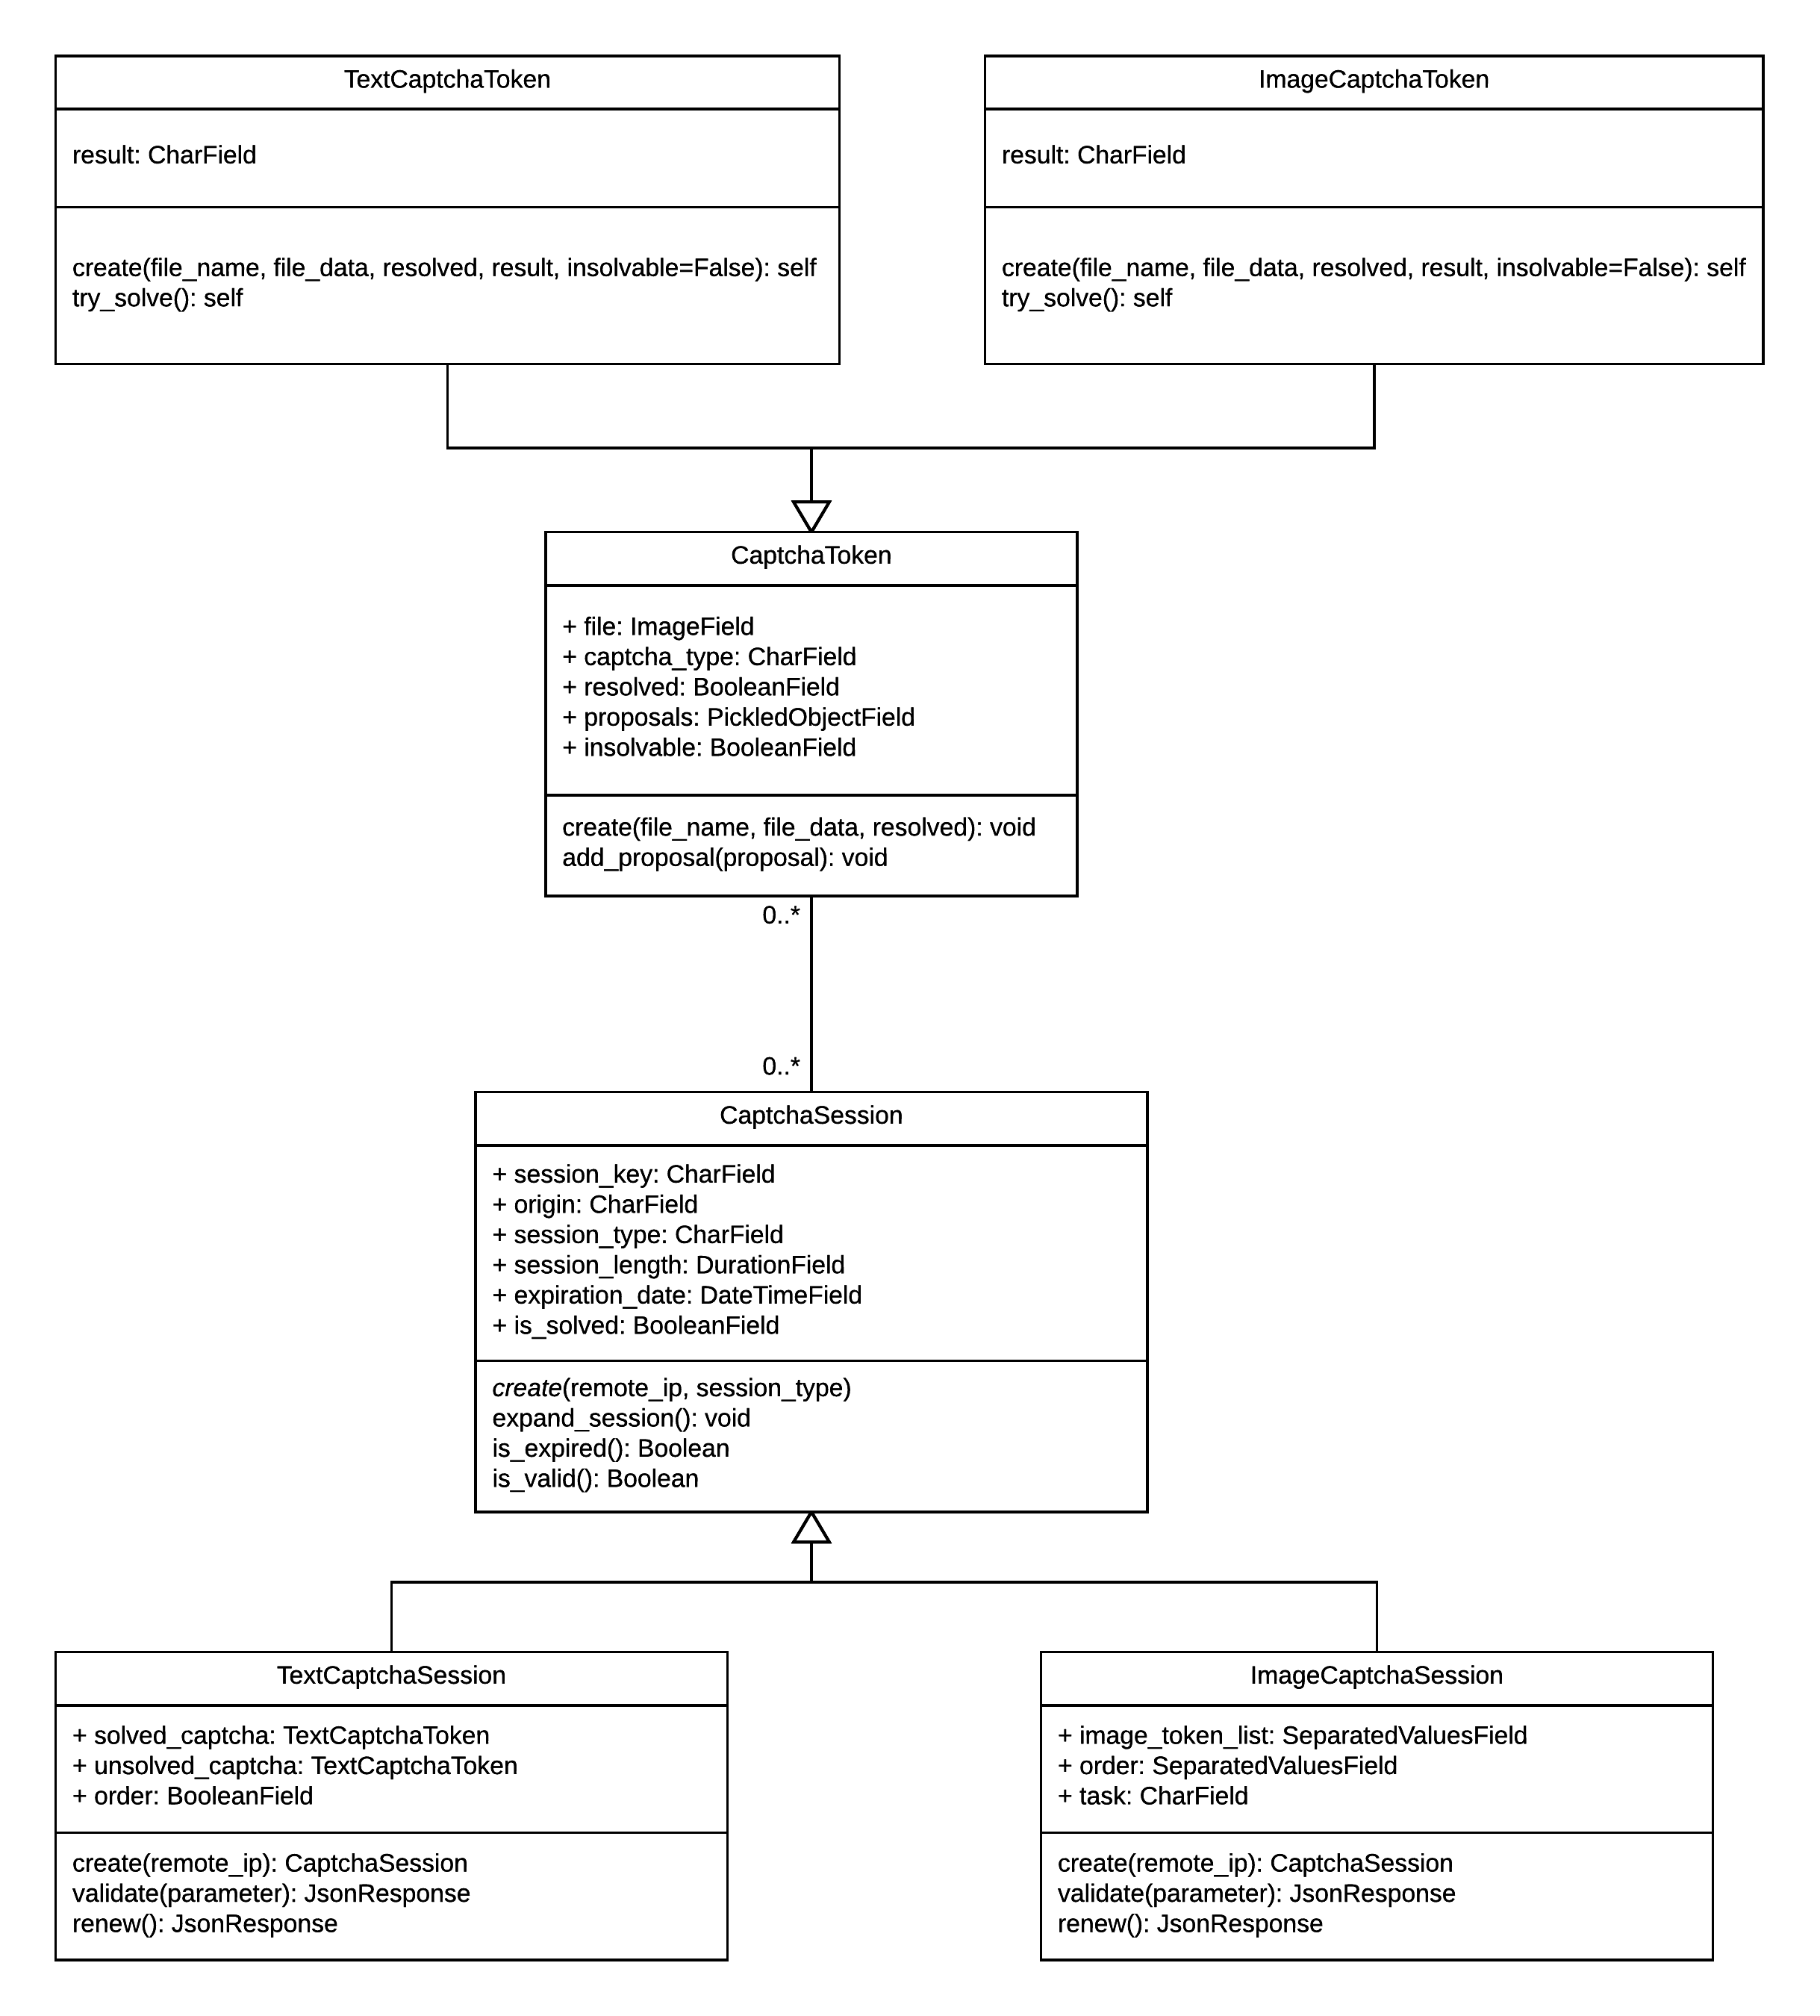
\includegraphics[width=1.1\linewidth]{content/figures/classdiagramm.png}
\caption{Class diagram representing the classes used for the generation of Captchas. The two main classes \emph{CaptchaToken} and \emph{CaptchaSession} are shown in the center. All other classes inherit from one of the superclasses.
}
\label{fig:classdia}
\end{figure}

The class \emph{CaptchaToken} represents a single image, that is part for a Captcha, e.g. a single word, that needs to be written down by the user in order to solve the Captcha. The class \emph{CaptchaSession} represents a complete Captcha challenge a user has to solve, e.g. writing down the words shown on all images. Each type of Captcha challenge provided by the service is represented by a subclass of \emph{CaptchaSession} and \emph{CaptchaToken}. Currently two kinds of Captchas, ImageCaptchas and TextCaptchas, are supported. 


All that needs to be done for implementing a new type of Captcha challenge is to create a new subclass for \emph{CaptchaToken} and \emph{CaptchaSession} and implement specific functionality in these subclasses. Which methods and attributes need to be added in the new subclasses is listed in the ``Attributes and Methods implemented in the subclass''-paragraph.

All instances of a \emph{CaptchaToken} or \emph{CaptchaSession} are saved in the \verb|db.sqlite3|-Database. 

\clearpage
\subsubsection{CaptchaToken}

The class \emph{CaptchaToken} is the basic unit of the Captcha service. Data, which is supposed to be labeled by the Captcha service is saved as a \emph{CaptchaToken}. Multiple \emph{CaptchaTokens} are combined to a Captcha challenge, when a new \emph{CaptchaSession} is created.

\paragraph{Attributes and Methods implemented in the superclass} \mbox{} \\
Attributes:

\begin{itemize}
\item \verb|file|: Image, that is represented by the CaptchaToken.
\item \verb|captcha_type|: String, that defines the type of Captcha the token can be used for. Currently ``text'' for TextCaptchas and ``image'' for ImageCaptchas are supported.
\item \verb|resolved|: Boolean, that indicates, if the solution for a \emph{CaptchaToken} is known or not. A \verb|0| means the token is unsolved and a \verb|1| means the Token is solved.
\item \verb|proposals|: Dictionary, that stores the possible solutions suggested by users of the Captcha service and how often each solution was suggested.
\item \verb|insolvable|: Boolean which indicates, that a token is not solvable by clients of the Captcha service. This value is set to \verb|True|, if there are many proposals for a \emph{CaptchaToken} without one proposal having the majority of the votes. For more information see \hyperref[sec:solving_algorithm]{section 6 (solving algorithm)}.
\end{itemize}

Methods:

\begin{itemize}
\item \verb|create(file_name, file_data, resolved)|: Responsible for basic configuration, that need to be done for all kinds of tokens, when they are created. Only used for super-calls in the \verb|create()|-method of subclasses.
\item \verb|add_proposals(proposal)|: Adds a new suggested solution to the \verb|proposals|-dictionary, or increments the counter for an already suggested proposal.
\end{itemize}

\paragraph{Attributes and Methods implemented in the subclass} \mbox{} \\
Attributes: 

\begin{itemize}
\item \verb|result|: Saves the correct solution for a token. Data type differs between different subclasses, e.g. \emph{TextCaptchaToken} saves a string and \emph{ImageCaptchaToken} saves a boolean.
\end{itemize}

Methods:

\begin{itemize}
\item \verb|create(file_name, file_data, resolved, result, insolvable=False)|: Responsible for configuration of all attributes of the \emph{CaptchaToken}. Returns a \emph{CaptchaToken}.
\item \verb|try_solve|: Responsible for finding the correct solution for a \emph{CaptchaToken} based on the values saved in the \verb|proposals|-attribute.
\end{itemize}

\clearpage
\subsubsection{CaptchaSession}

Represents an instance of a Captcha challenge, that needs to be solved by a certain client. A \emph{CaptchaSession} consists of multiple \emph{CaptchaTokens}, that are chosen randomly in order to create different challenges dynamically. Each Session corresponds to one of the supported types of \emph{CaptchaTokens}. The tokens chosen are a mix of solved and unsolved tokens, in order to make it possible to validate the session and label new data.

\paragraph{Attributes and Methods implemented in the superclass} \mbox{} \\
Attributes:

\begin{itemize}
\item \verb|session_key|: String, that serves as primary key to identify each session. 
\item \verb|origin|: String, that holds the IP address that requested the Captcha challenge. It is used to match requests made by the client to the corresponding session.
\item \verb|session_type|: String, that defines the kind of Captcha challenge, the client has to solve. Currently ``text'' for TextCaptchas and ``image'' for ImageCaptchas are supported.
\item \verb|session_length|: Timedelta, that stores the amount of time in which a session can be validated. The default value is 30 minutes, which is initialised in the \verb|create()| method of \emph{CaptchaSession}.
\item \verb|expiration_date|: Datetime, that stores the date, after which a \emph{CaptchaSession} can not be validated anymore.
\item \verb|is_solved|: Boolean, that stores if a \emph{CaptchaSession} was already solved by the client.
\end{itemize}

Methods:

\begin{itemize} 
\item \verb|create(remote_ip, session_type)|: Responsible for basic creation of a \emph{CaptchaSession} of the requested type for the given IP address. Only used for super-calls in the \verb|create()|-method of subclasses.
\item \verb|expand_session()|: Responsible for changing the \verb|expiration_date| of a \emph{CaptchaSession} so that the session is valid for another \verb|session_length|.
\item \verb|is_expired()|: Responsible for checking, if a session is expired. Returns \verb|True| when the current date is before the \verb|expiration_date|.
\item \verb|is_valid()|: Responsible for checking, if a \emph{CaptchaSession} was successfully validated by a client and is not expired. In that case \verb|True| is returned.
\end{itemize}

\paragraph{Attributes and Methods implemented in the subclass} \mbox{} \\
Attributes:

Each session needs to store the tokens, which were used for creating the session as well as additional information, that is needed for validating the answer given by the client. This can differ for every Captcha type. 

TextCaptchaSession:

\begin{itemize} 
\item \verb|solved_captcha_token|: \emph{TextCaptchaToken}, that is already solved and is used as a control word for the session.
\item \verb|unsolved_captcha_token|: \emph{TextCaptchaToken}, that is not solved and shall be identified by the client.
\item \verb|order|: Boolean indicating the order, in which the two tokens are displayed to the client (0 -> solved, unsolved 1 -> unsolved, solved). It is needed to map the answers given by the client to the right tokens.
\end{itemize}


ImageCaptchaSession:

\begin{itemize}
\item \verb|image_token_list|: List of \emph{ImageCaptchaTokens}, where all tokens used for the session are saved.
\item \verb|order|: List of Booleans, that indicates, which token in the \verb|image_token_list| is solved (0 -> unsolved, 1-> solved).
\item \verb|task|: String, that saves the object that should be detected in the Captcha challenge, e.g. cat, if cats should be identified.
\end{itemize}

Methods: 

\begin{itemize}
\item \verb|create(remote_ip)|: Responsible for creating a \emph{CaptchaSession} and returning the created session to the corresponding \verb|view|, and a JsonResponse with the parameters needed to render the Captcha challenge in the front end (e.g. urls of pictures that are shown in the challenge). Depending on the type of the \emph{CaptchaSession}, the function chooses a mix of multiple \emph{CaptchaTokens} with some of them being unsolved and some of them being solved. The unsolved \emph{CaptchaTokens} are data that shall be labeled and the solved \emph{CaptchaTokens} are used for checking, if the answer for the \emph{CaptchaSession} is correct. 
\item \verb|validate(parameters)|: Responsible for validating the solution for a CaptchaSession and returning the created session to the corresponding \verb|view|. The solution suggested by the client is included in the parameters. The method checks, if the suggested solutions matches the solution for the solved \emph{CaptchaTokens}. If the solution given by the client is correct, \verb|proposals| are added for the unsolved \emph{CaptchaTokens} and \verb|try_solve()| is called on these tokens. If the solution is false new \emph{CaptchaTokens} are chosen for the \emph{CaptchaSession} to prevent brute forcing. Returns a JsonResponse with information, whether the session is valid or not and a list of image-URLs that shall be rendered in the session.
\item \verb|renew()|: Responsible for exchanging the \emph{CaptchaTokens} of a \emph{CaptchaSession}, to create a new challenge or the same session. Returns a JsonResponse of the updated information needed to render the session in the front end.
\end{itemize}

\clearpage
\paragraph{Session length and expiration} \mbox{} \\

A \emph{CaptchaSession} expires after a certain amount of time, in order to prevent replay attacks. For this reason \verb|is_valid()| always returns false after the expiration date is over. The \emph{CaptchaSession} however remains in the database indefintely, because Django does not provide an elegant method to automatically delete session after expiry. Therefore the CaptchaService provides a Django command, which is called \verb|delete_timeouted_sessions| and on execution removes all timed out \emph{CaptchaSessions} in the Database. This can be paired with a cron job so that timed out sessions will be deleted in short intervals. 

\clearpage
\subsection{Views (views.py)}

The views handle POST- and GET-Requests made by the Client, third party web application and the web interface. List of Requests handled by views:

\begin{itemize}
\item \verb|request(request)|: GET-Request called by the client, when a new session is requested. Chooses a type for the session randomly, calls create-Method for the session implemented in \verb|models.py| and directs the response of session.create() to the client.
\item \verb|validate(request)|: POST-Request called by the client, when a solution for a Captcha challenge is submitted. Retrieves the the corresponding \emph{CaptchaSession} from the database, calls the validate-Method of the session and directs the response to the client.
\item \verb|renew(request)|: POST-Request called by the client, when a new challenge for an existing \emph{CaptchaSession} shall be provided. Retrieves the corresponding \emph{CaptchaSession} from the database, calls the renew-Method of the session and directs the response to the client.
\item \verb|upload(request)|: POST-Request called by the web interface, when new files are uploaded to the Captcha service. Extracts the files from the zip-file and creates tokens corresponding to the provided data.
\item \verb|download(request)|: GET-Request called by the web interface, to retrieve tokens and solutions from the database. Collects \emph{CaptchaTokens}, that meet the requirements specified in the web interface, compresses them to a zip-file and returns the file.
\item \verb|getTask(request)|: GET-Request called by the web interface, to get all possible tasks for an \emph{ImageCaptchaSession}. Gets all tasks from the database and returns them as a list in a JsonResponse.
\item \verb|validate_solved_session(request)|: GET-Request called by the third party web application, to check if a \emph{CaptchaSession} was successfully validated by a client. This prevents clients from being able to bypass the Captcha challenge.
\end{itemize}

\clearpage
